% !TEX TS-program = pdflatex
% !TEX encoding = UTF-8 Unicode
% !TEX root = ../2018-03-26-papa-vitres-de-son.tex

%************************************************
\chapter{La ricerca dei materiali (elettromeccanici)}
\label{chp:La ricerca dei materiali (elettromeccanici)}
%************************************************

Le molle prese in esame sono state a (trazione) e a (compressione).
Dopo varie ricerche fatte anche su materiali presenti al CRM, la soluzione per l'esecuzione del pezzo è la seguente:

\begin{itemize}
\item{L'acciaio armonico è risultato il materiale migliore per il mio utilizzo perché a diametri bassi di filatura si possono avere grandi o piccoli diametri per le spire e il risultato non cambia.}
\item{Ogni molla, se ha un diametro compreso tra 0.1 e 0.2 cm, si ottiene una grande manovrabilità a livello di flessione e tensione. Da sottolineare che vanno utilizzate solo ed esclusivamente le \underline {Molle a Trazione}; perché in estensione hanno rigidità minime anche per lunghezze pari al doppio della loro lunghezza a riposo.}
\end{itemize}

Tipologia di molle utilizzate:

\begin{tabular}{cp{2cm}p{2cm}p{.2cm}p{2cm}} \textbf{MOLLA}&\textbf{DIAM.}&\textbf{LUNGH.}\\
\hline \textit{in centimetri} \\
\hline 5&2&20\\
\hline 4&1.2&20\\
\hline 3&1.5&20\\
\hline 2&0.8&8\\
\hline 1&0.6&8\\
\end{tabular}

Perimetro delle lastre:

\begin{tabular}{cp{2cm}p{2cm}p{.2cm}p{2cm}} \textbf{PIASTRA}&\textbf{LARGH.}&\textbf{LUNGH.}\\
\hline \textit{in centimetri} \\
\hline 1&2&20\\
\hline 2&1.2&20\\
\hline 3&1.5&20\\
\hline 4&0.8&8\\
\end{tabular}

\section{Progettazione e supporto di tiraggio}

% \begin{figure}[htbp]
%        \centering
%        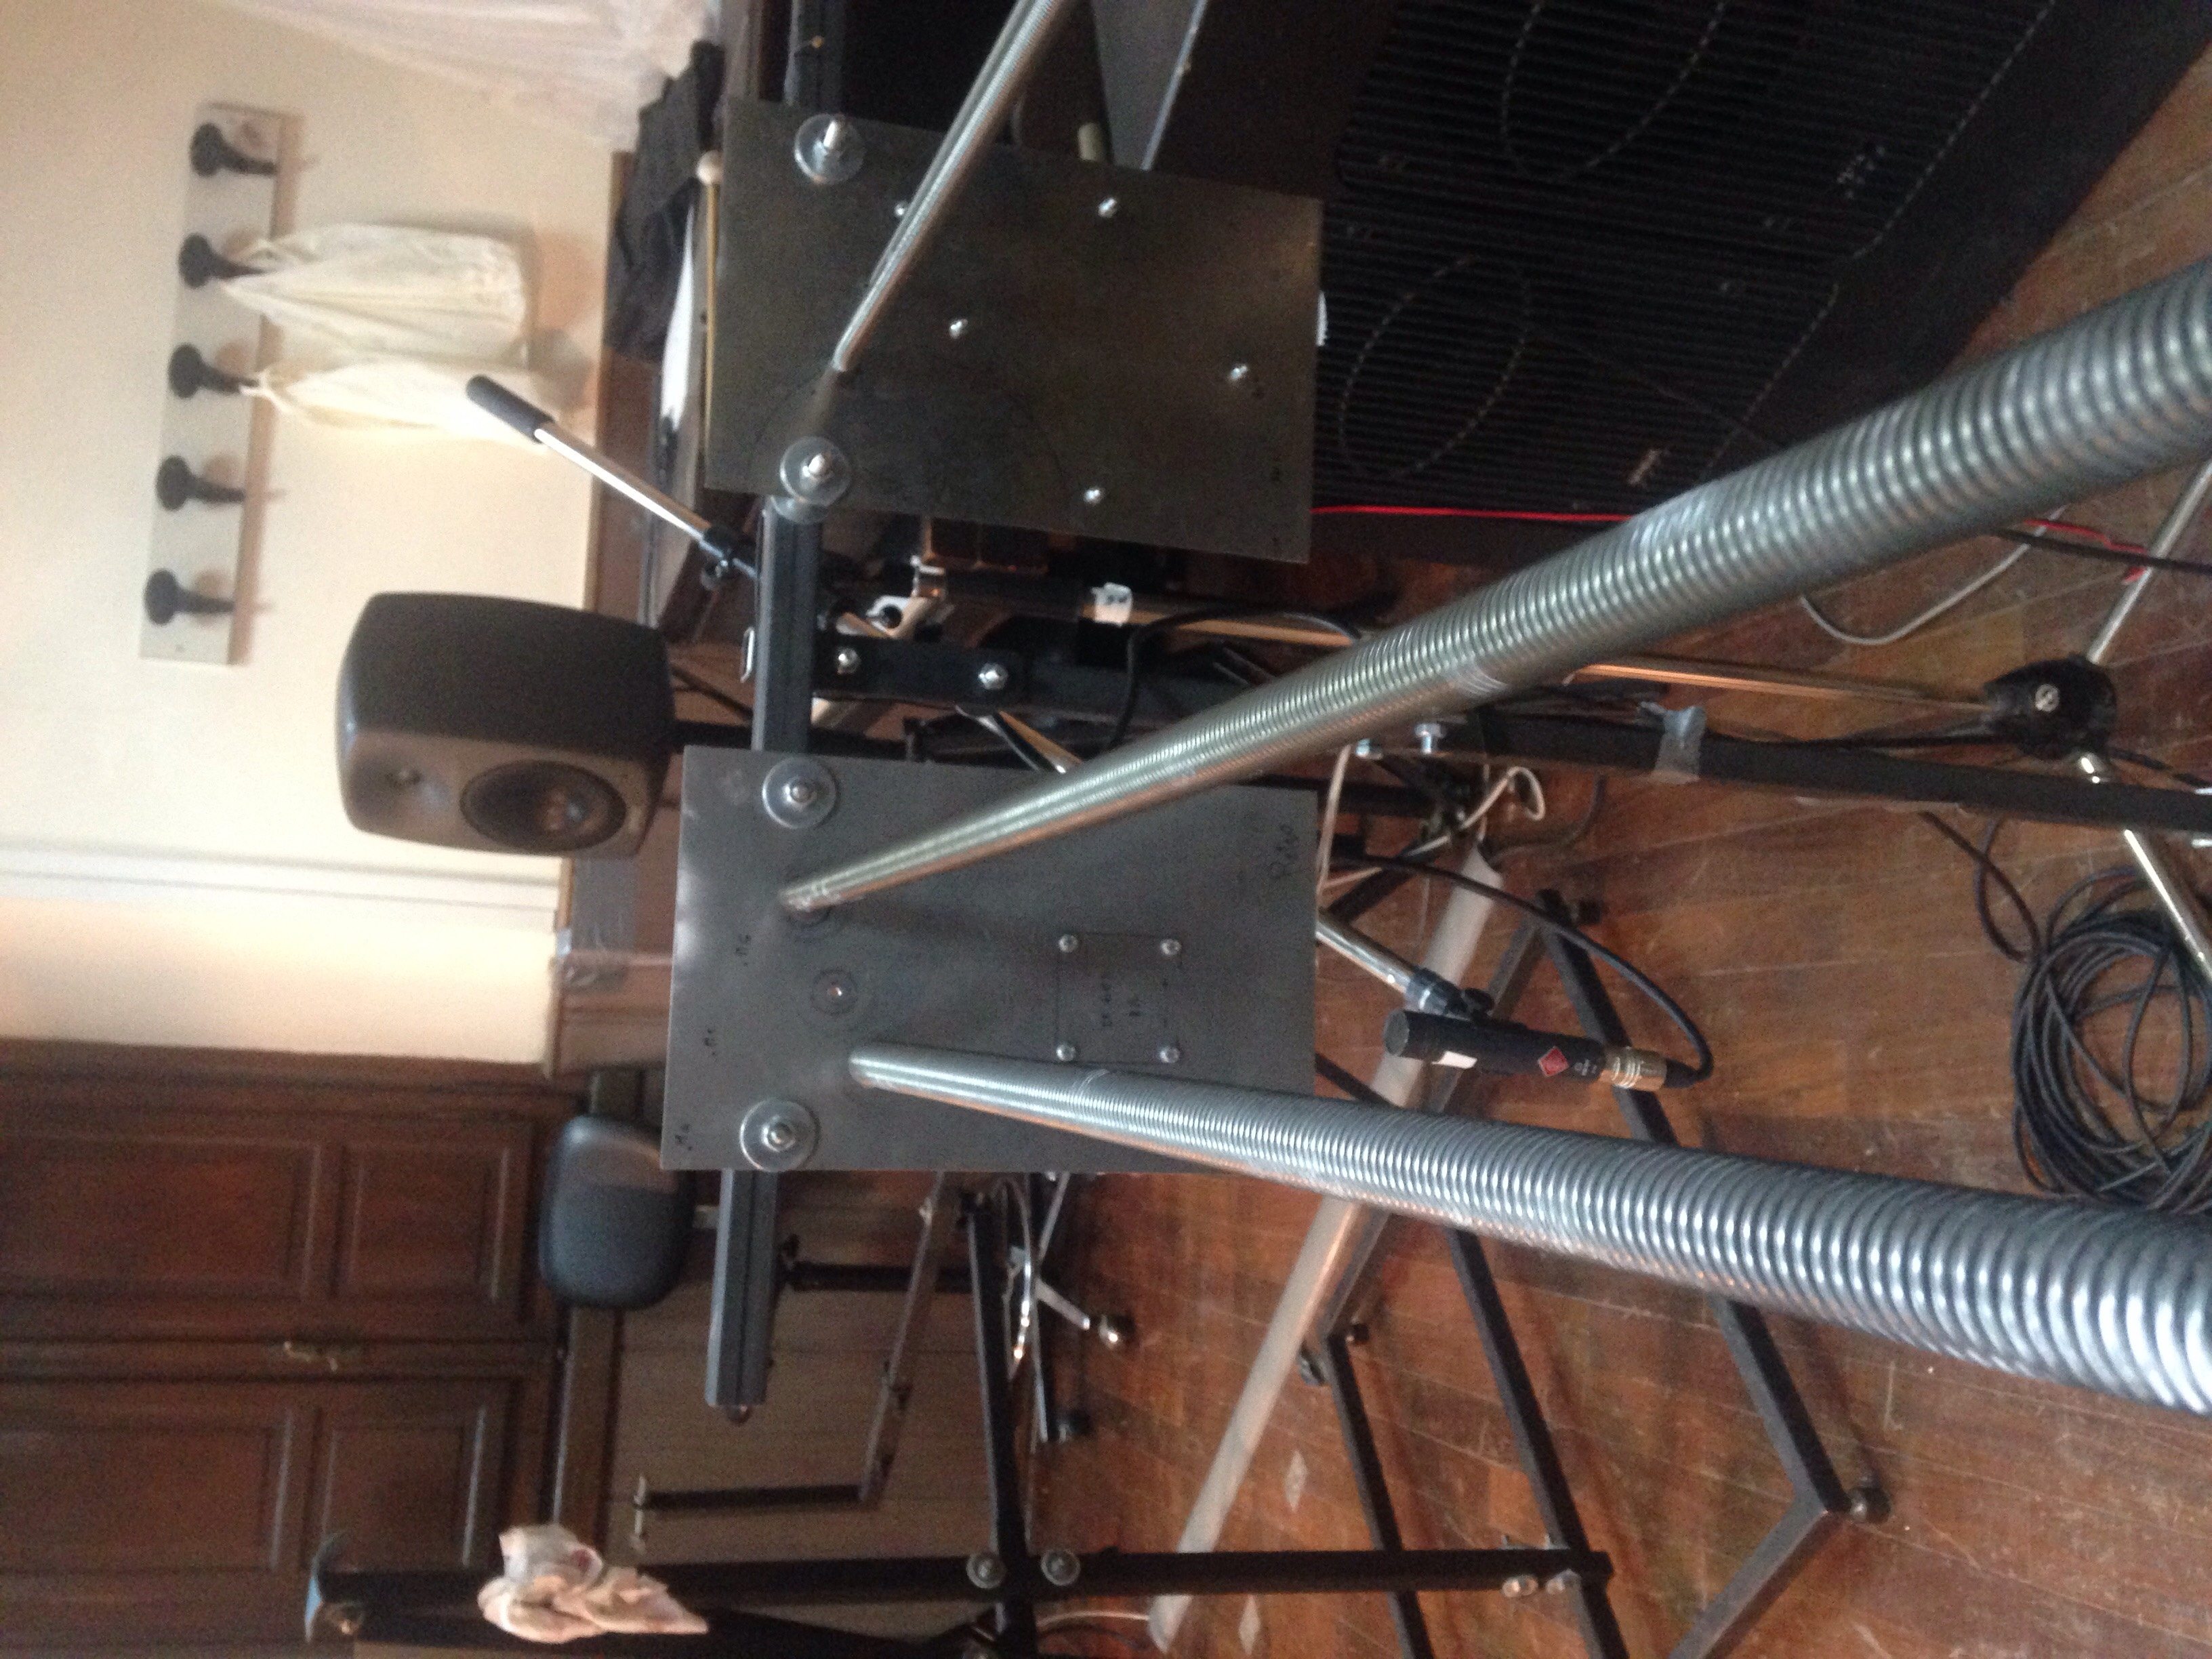
\includegraphics[height=6cm, width=5cm, angle=0,
%          keepaspectratio]{Spire2.jpg}
%\end{figure}
\begin{figure}[htbp]
\begin{center}
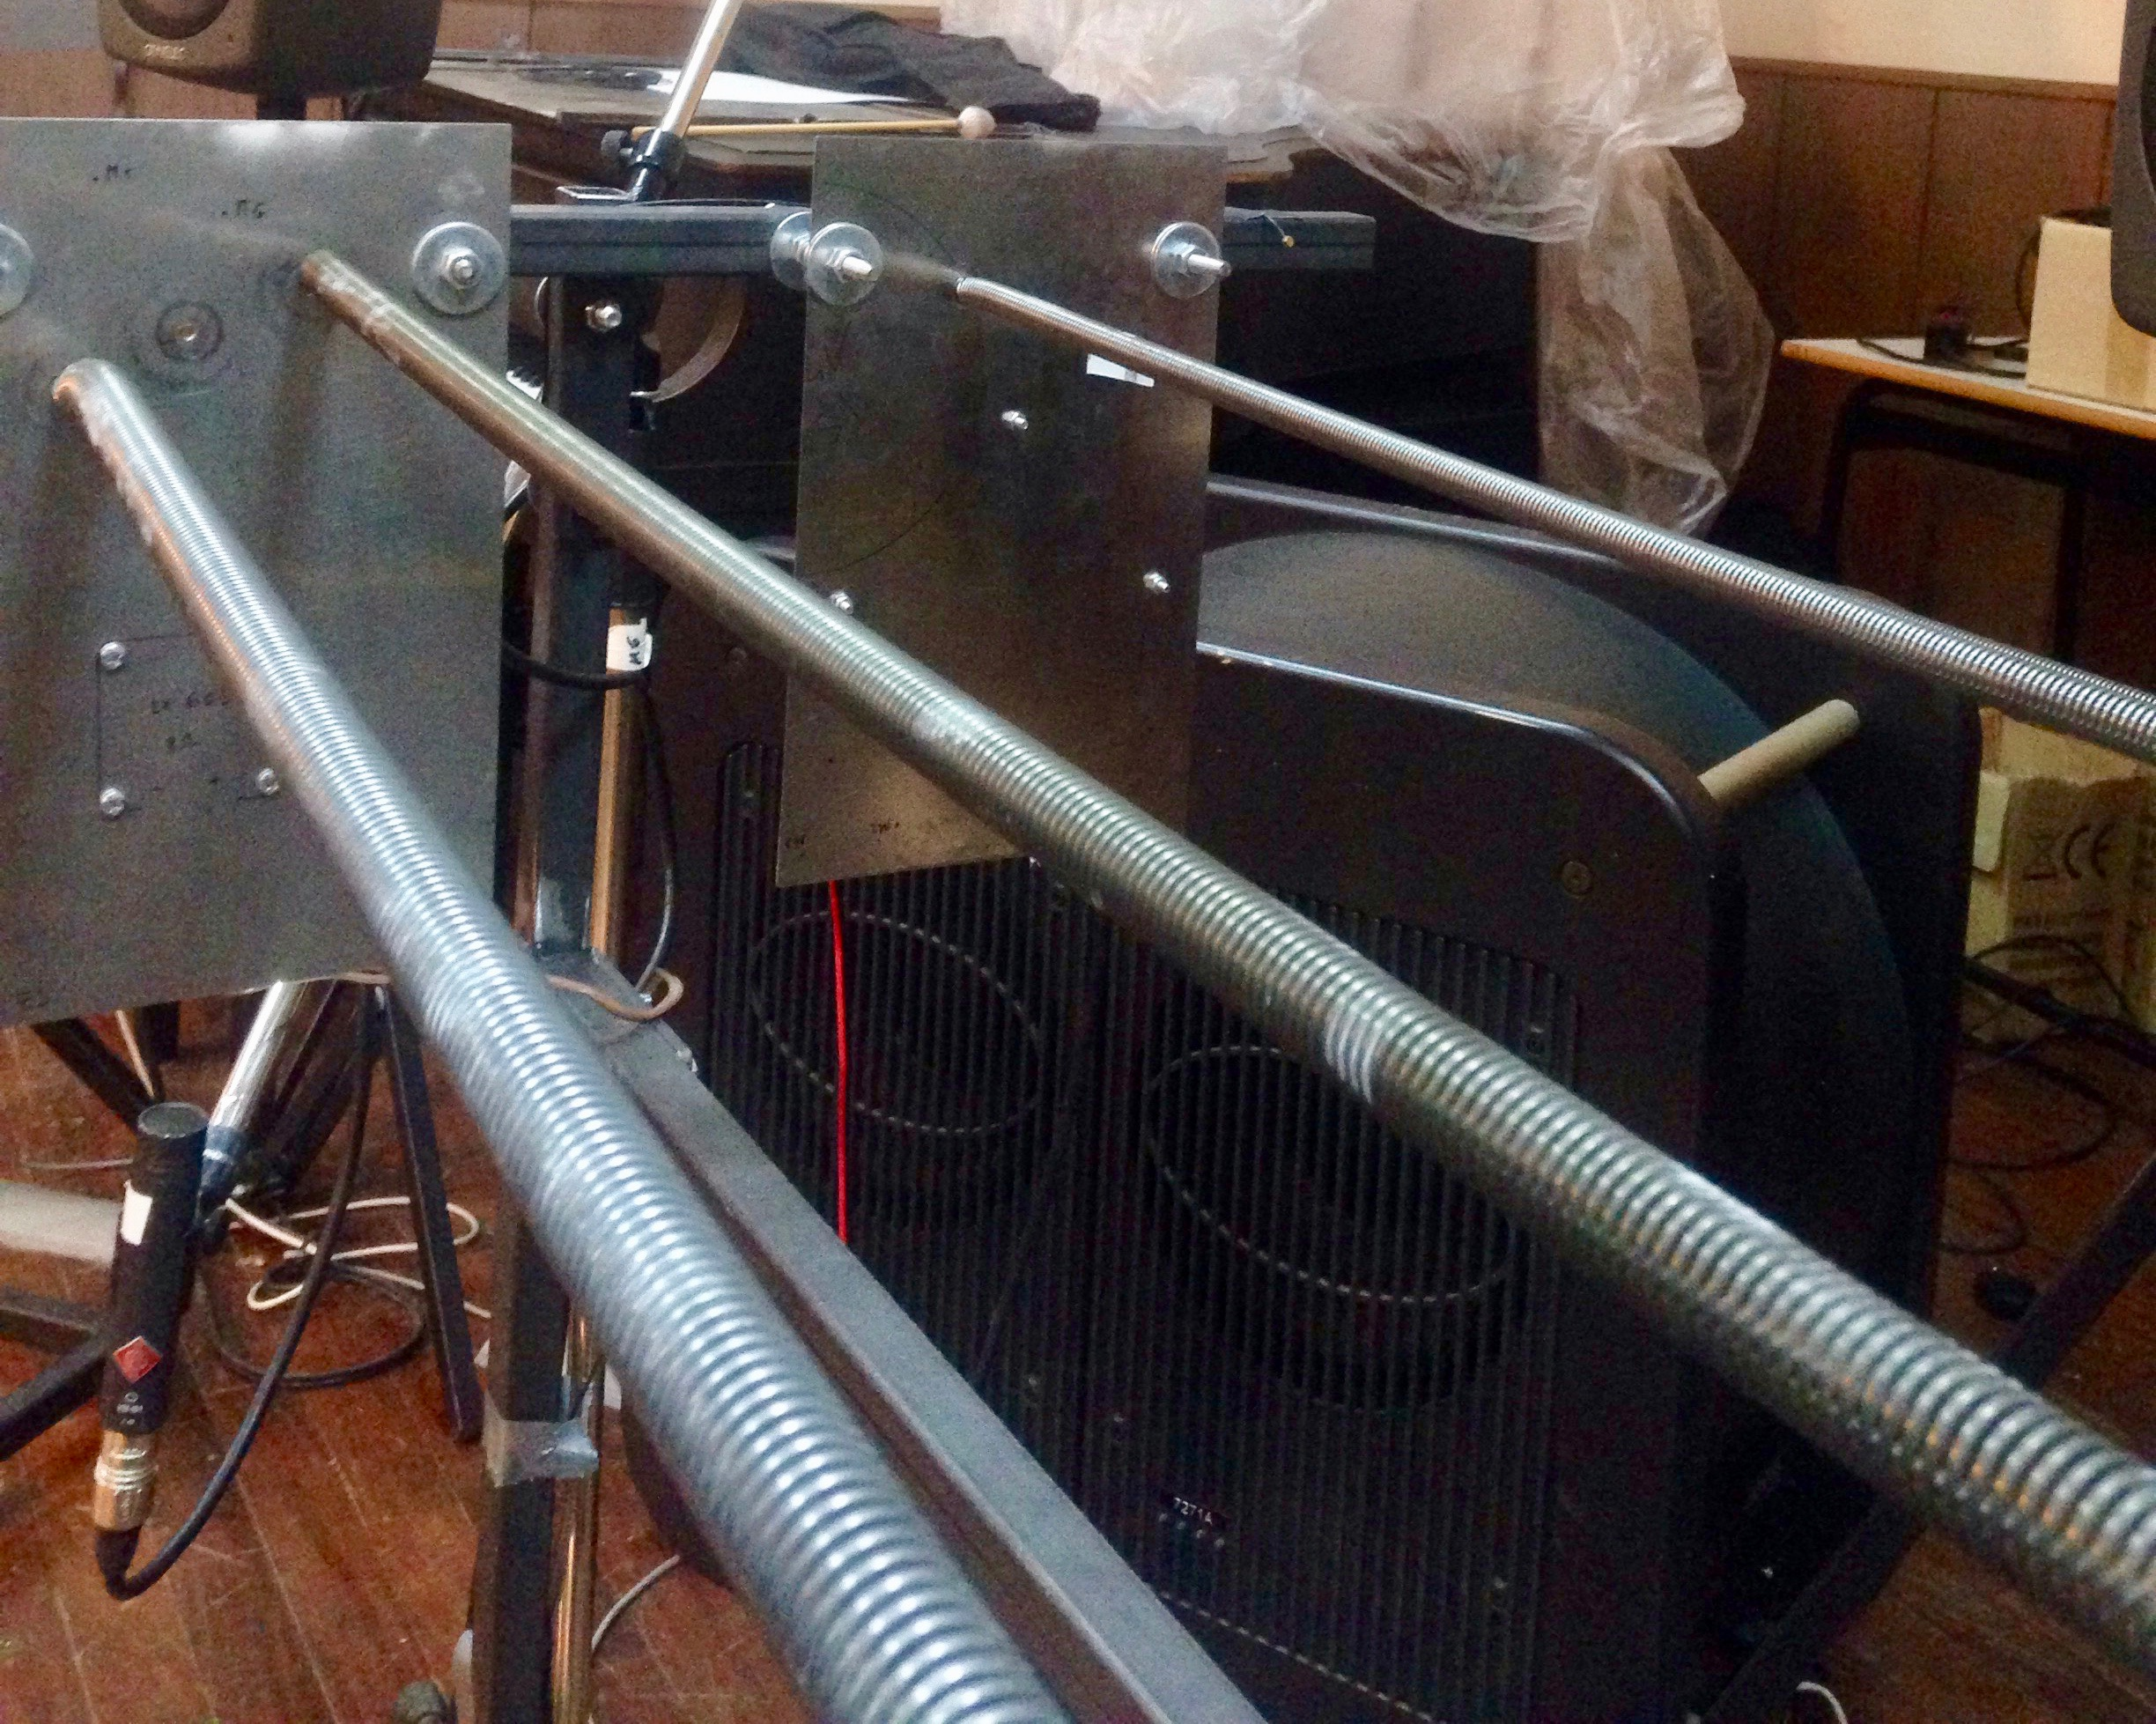
\includegraphics[width=.99\textwidth]{Spire3cc.jpg}
\caption{Particolare delle molle più esterne, quelle più gravi (Molla 4 e 5)}
\label{default}
\end{center}
\end{figure}
Le molle a trazione possono arrivare ad una forza di tiraggio pari anche a 100 chili. Per questo l'utilizzo di un basamento adeguato, creato su misura da un fabbro, è la soluzione a qualunque problema relativo al paragrafo successivo: il fissaggio di attuatori e molle.
Il basamento è stato creato, come scritto in precedenza, grazie all'aiuto di un assistente del Centro di Ricerche Musicali, Leonardo Mammozzetti, che ha visionato e modificato il progetto. Il supporto è in ferro e come in figura ... notiamo i punti di saldatura, segnati in verde. In basso a destra il nome degli attuatori utilizzati, la marca è Visaton.
\begin{figure}[htbp]
\begin{center}
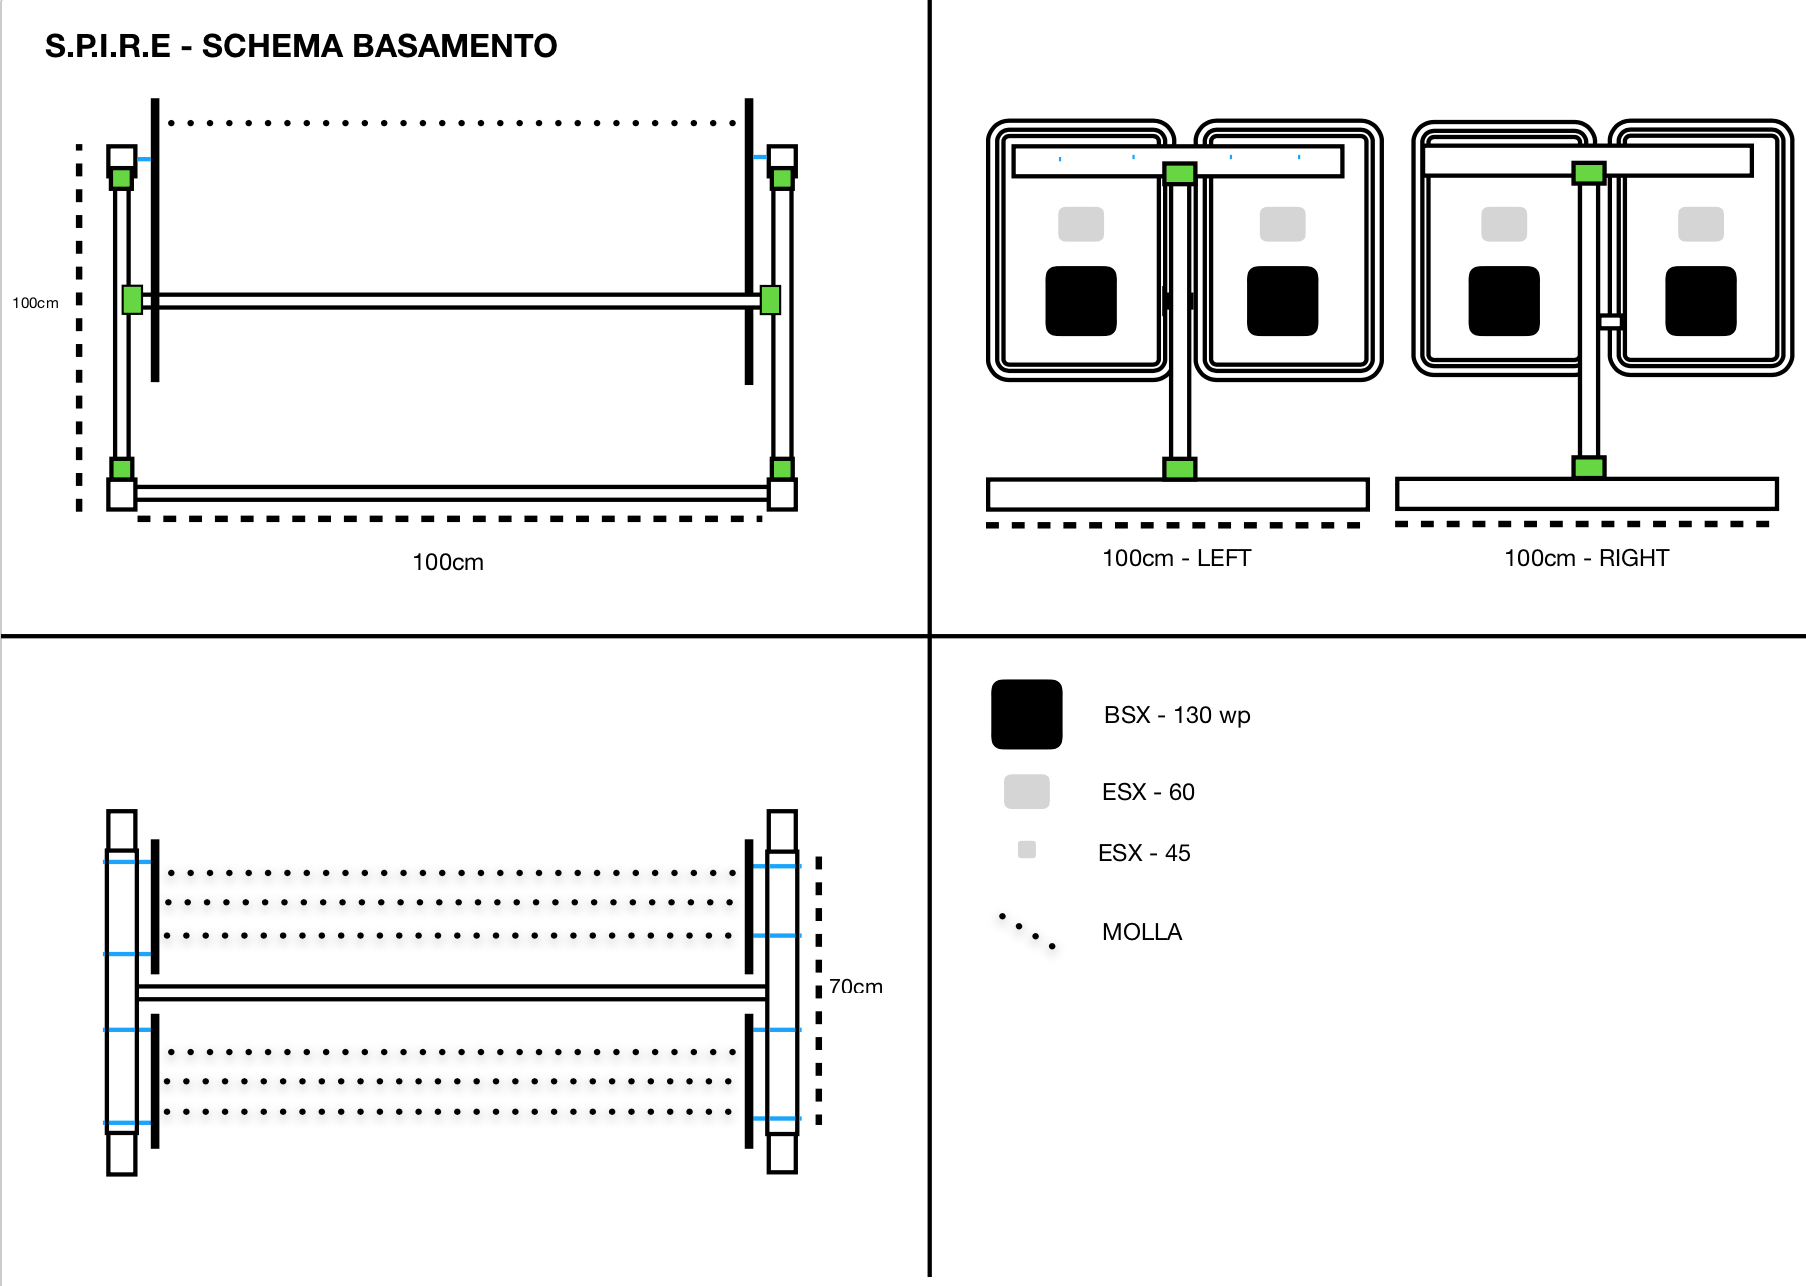
\includegraphics[width=.99\textwidth]{Basamento.jpg}
\caption{Basamento dello strumento}
\label{default}
\end{center}
\end{figure}
%\begin{figure}[htbp]
%        \centering
%        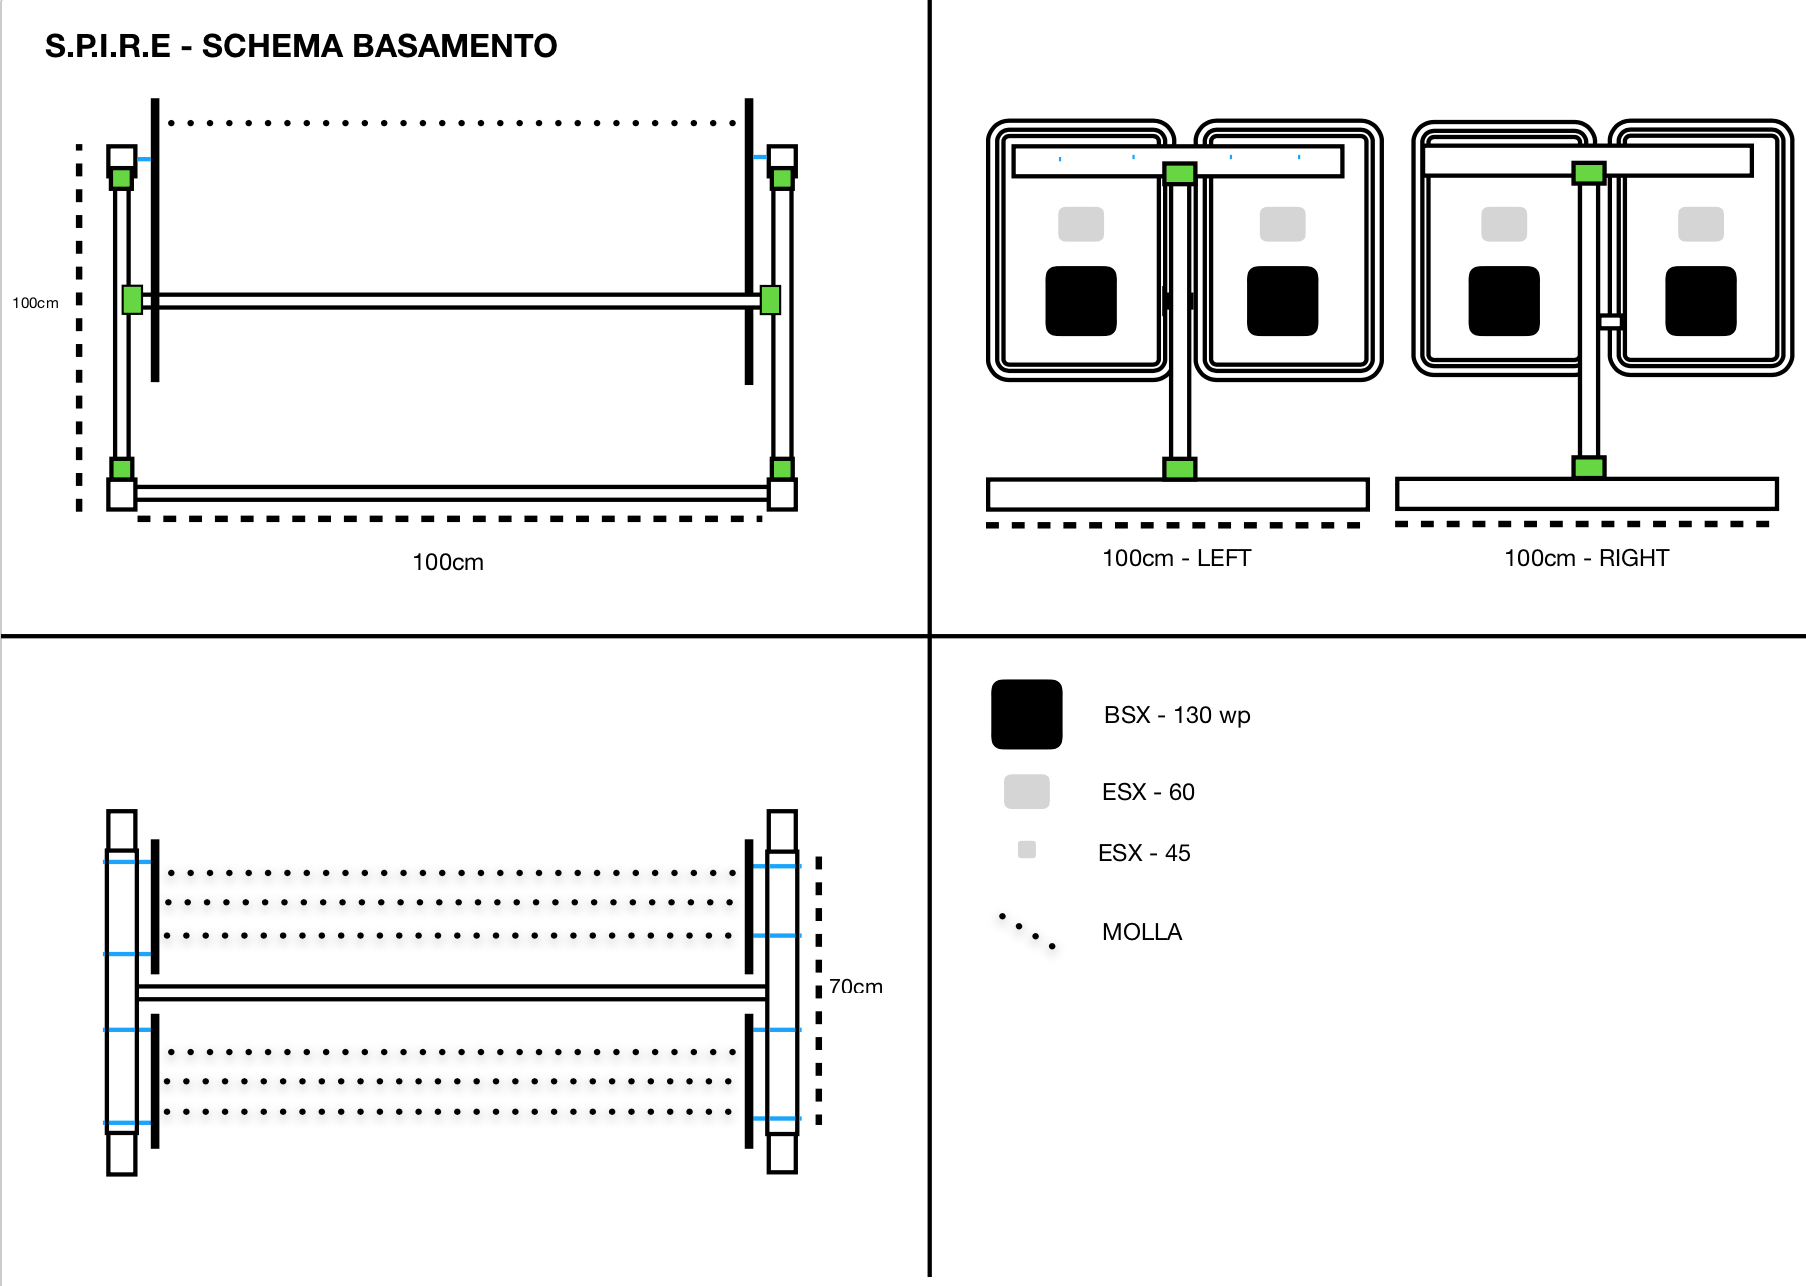
\includegraphics[height=15cm, width=15cm,
%          keepaspectratio]{Basamento.jpg}
%\end{figure}
Le molle a trazione sono state fissate come in figura, facendo dei buchi sulla lamiera e tese, tutto nella stessa lunghezza, per rendere possibile uno studio omogeneo su materiali diversi che rispondono diversamente al tocco e all'eccitazione mediante attuatori.\\
Si è notato che ogni molla si comporta differentemente a seconda del diametro delle spire, della robustezza del materiale e, ovviamente, del diametro del cavo in acciaio armonico.
%
%\begin{figure}[htbp]
%        \centering
%        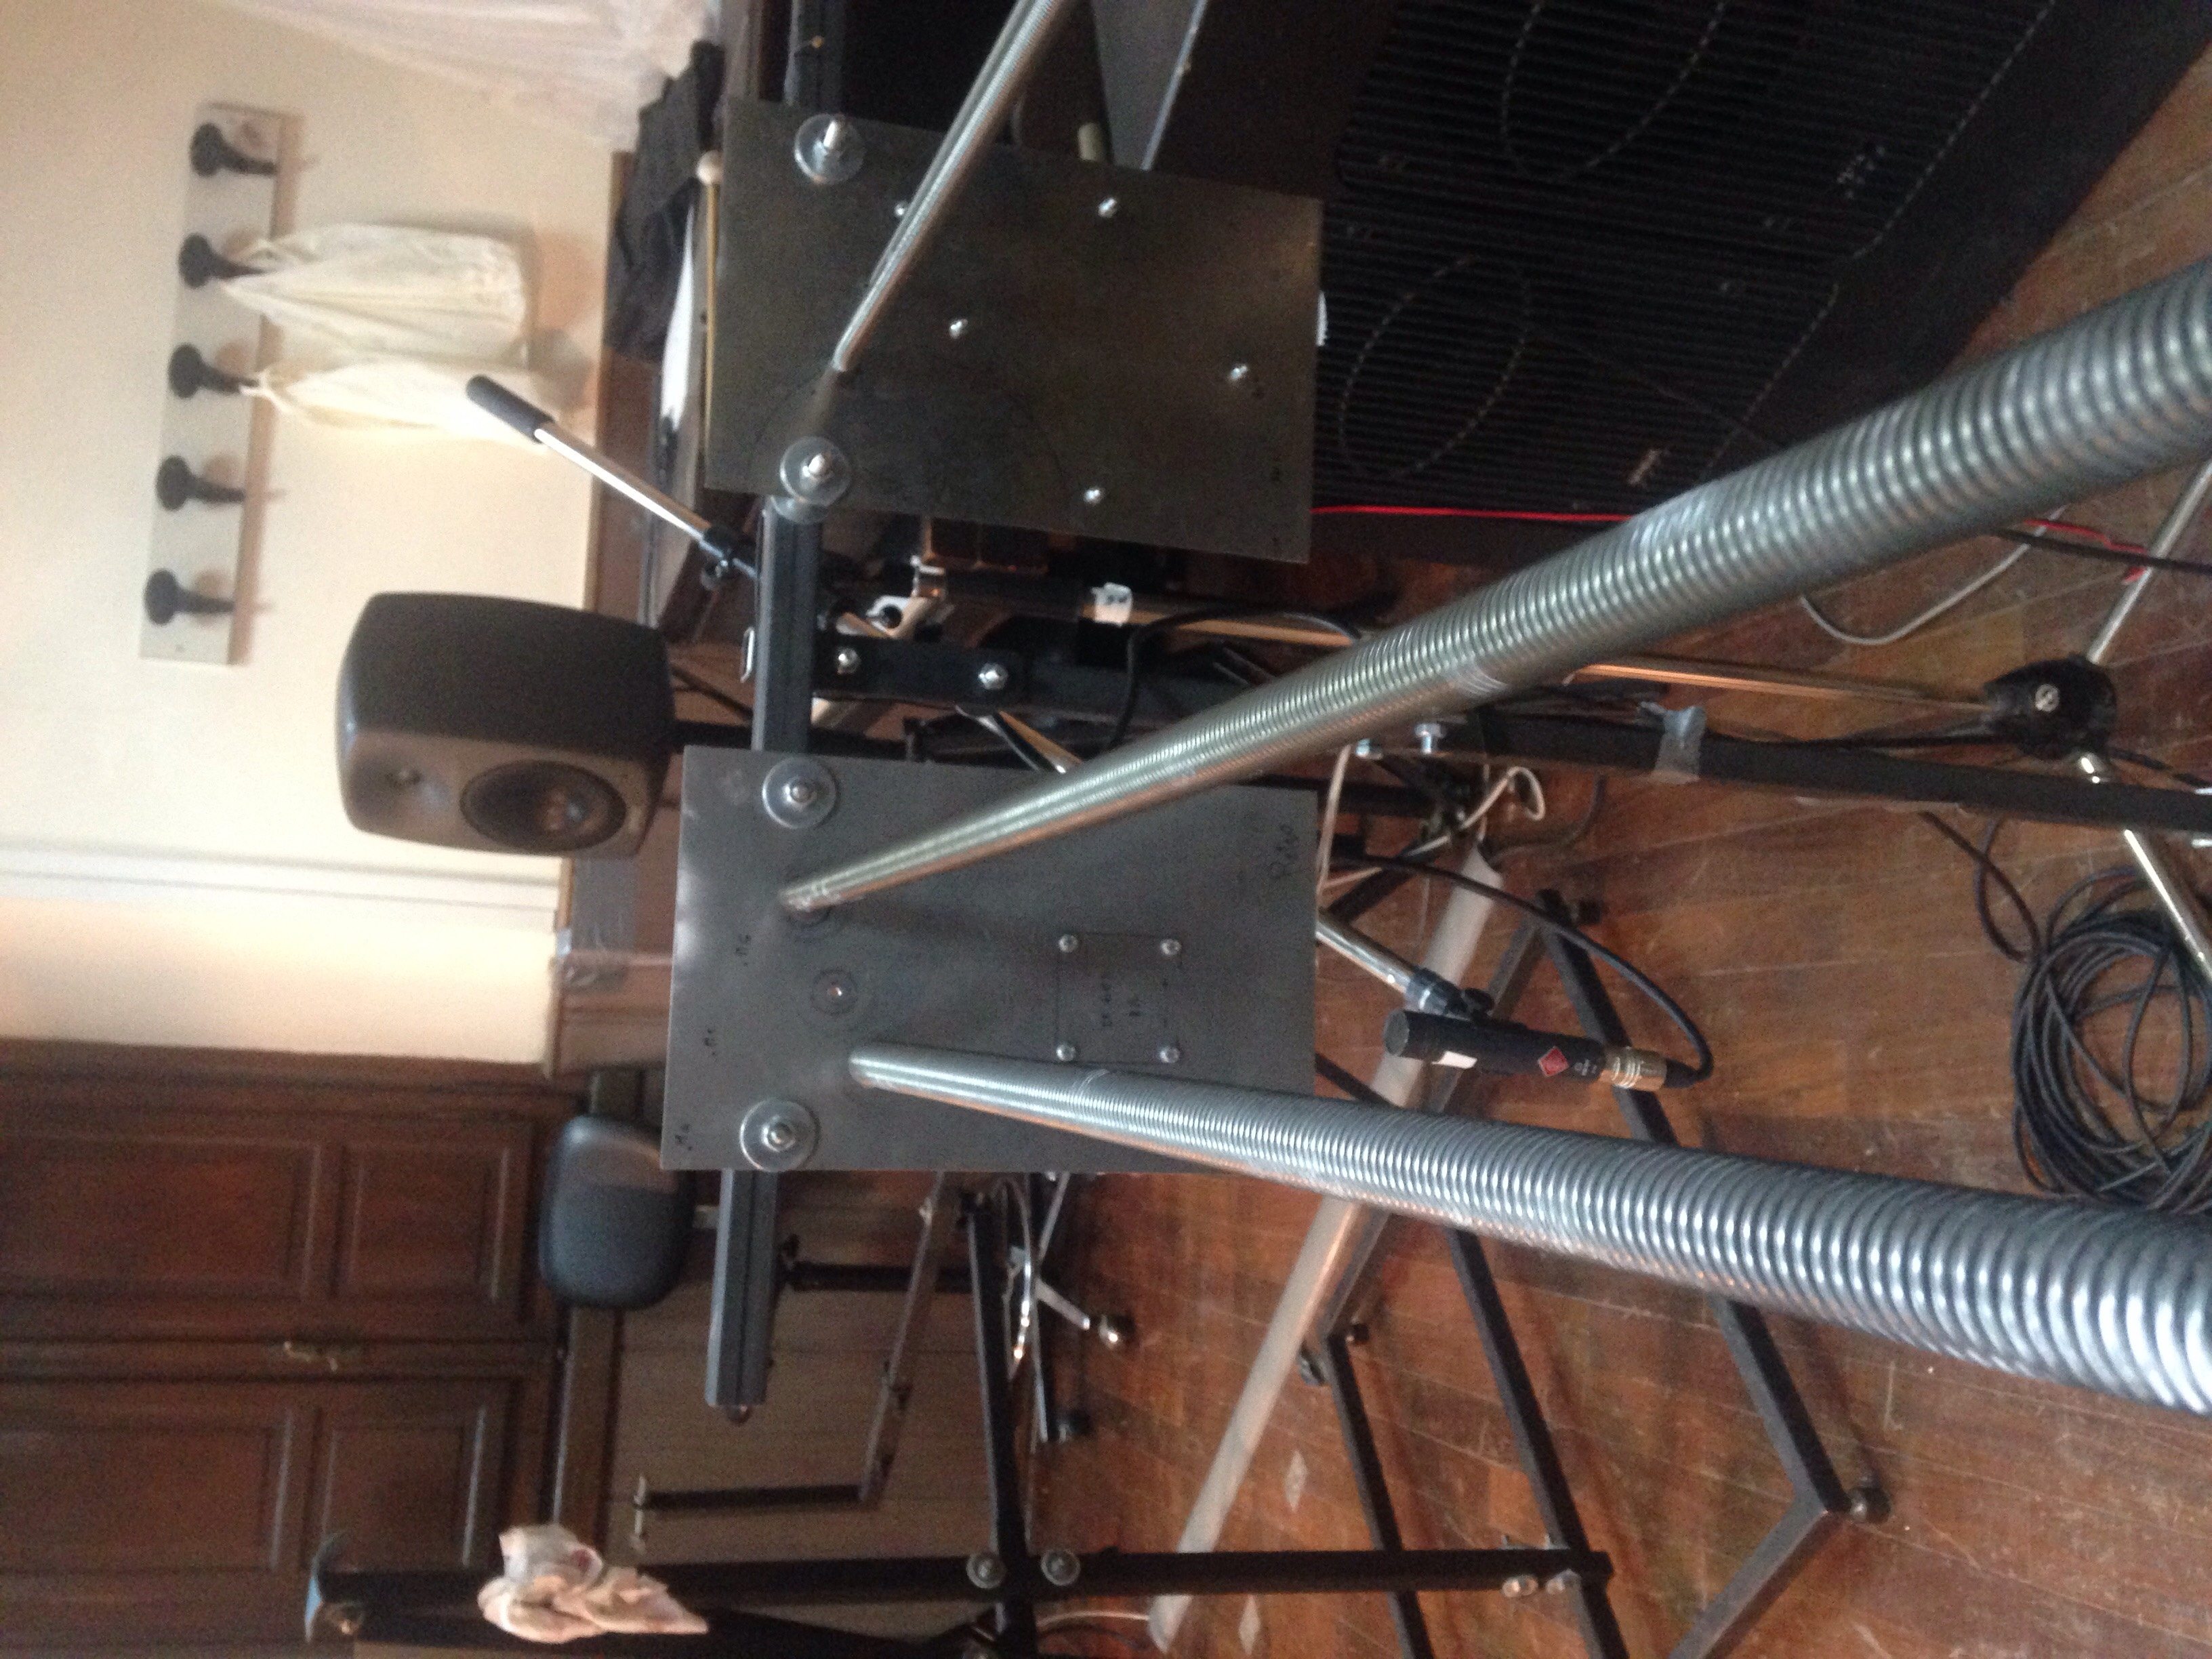
\includegraphics[height=6cm, width=5cm, angle=0,
%          keepaspectratio]{Spire2.jpg}
%\end{figure}

Tutti gli studi sono stati fatti su acciaio armonico o acciaio inox. Due sono i fattori che regolano il funzionamento della molla a trazione:

\begin{enumerate}
\item{Diametro del filo}
\item{Larghezza del diametro esterno (\textit{spira})}
\end{enumerate}

Il diametro del filo (1.) unito alla larghezza del diametro esterno (2.) rendono possibile il cambiamento della qualità della flessione della molla. Anche il numero di spire agisce sulla flessione della molla.

\section{Fissaggio Molle e attuatori}

Un basamento unisce quattro placche di metallo che montano tre molle ciascuna, tese per la lunghezza paritaria di 80 centimetri. Il basamento è in ferro, le placche rettangolari, in acciaio armonico, le molle in ferro armonico. Nel primissimo prototipo una delle molle, la numero 4\footnote{guardare la \textit{Legenda} sita in partitura} era in acciaio inox, ma non avendo ottenuto i risultati acustici sperati, ho deciso di cambiarla. 
\begin{figure}[htbp]
\begin{center}
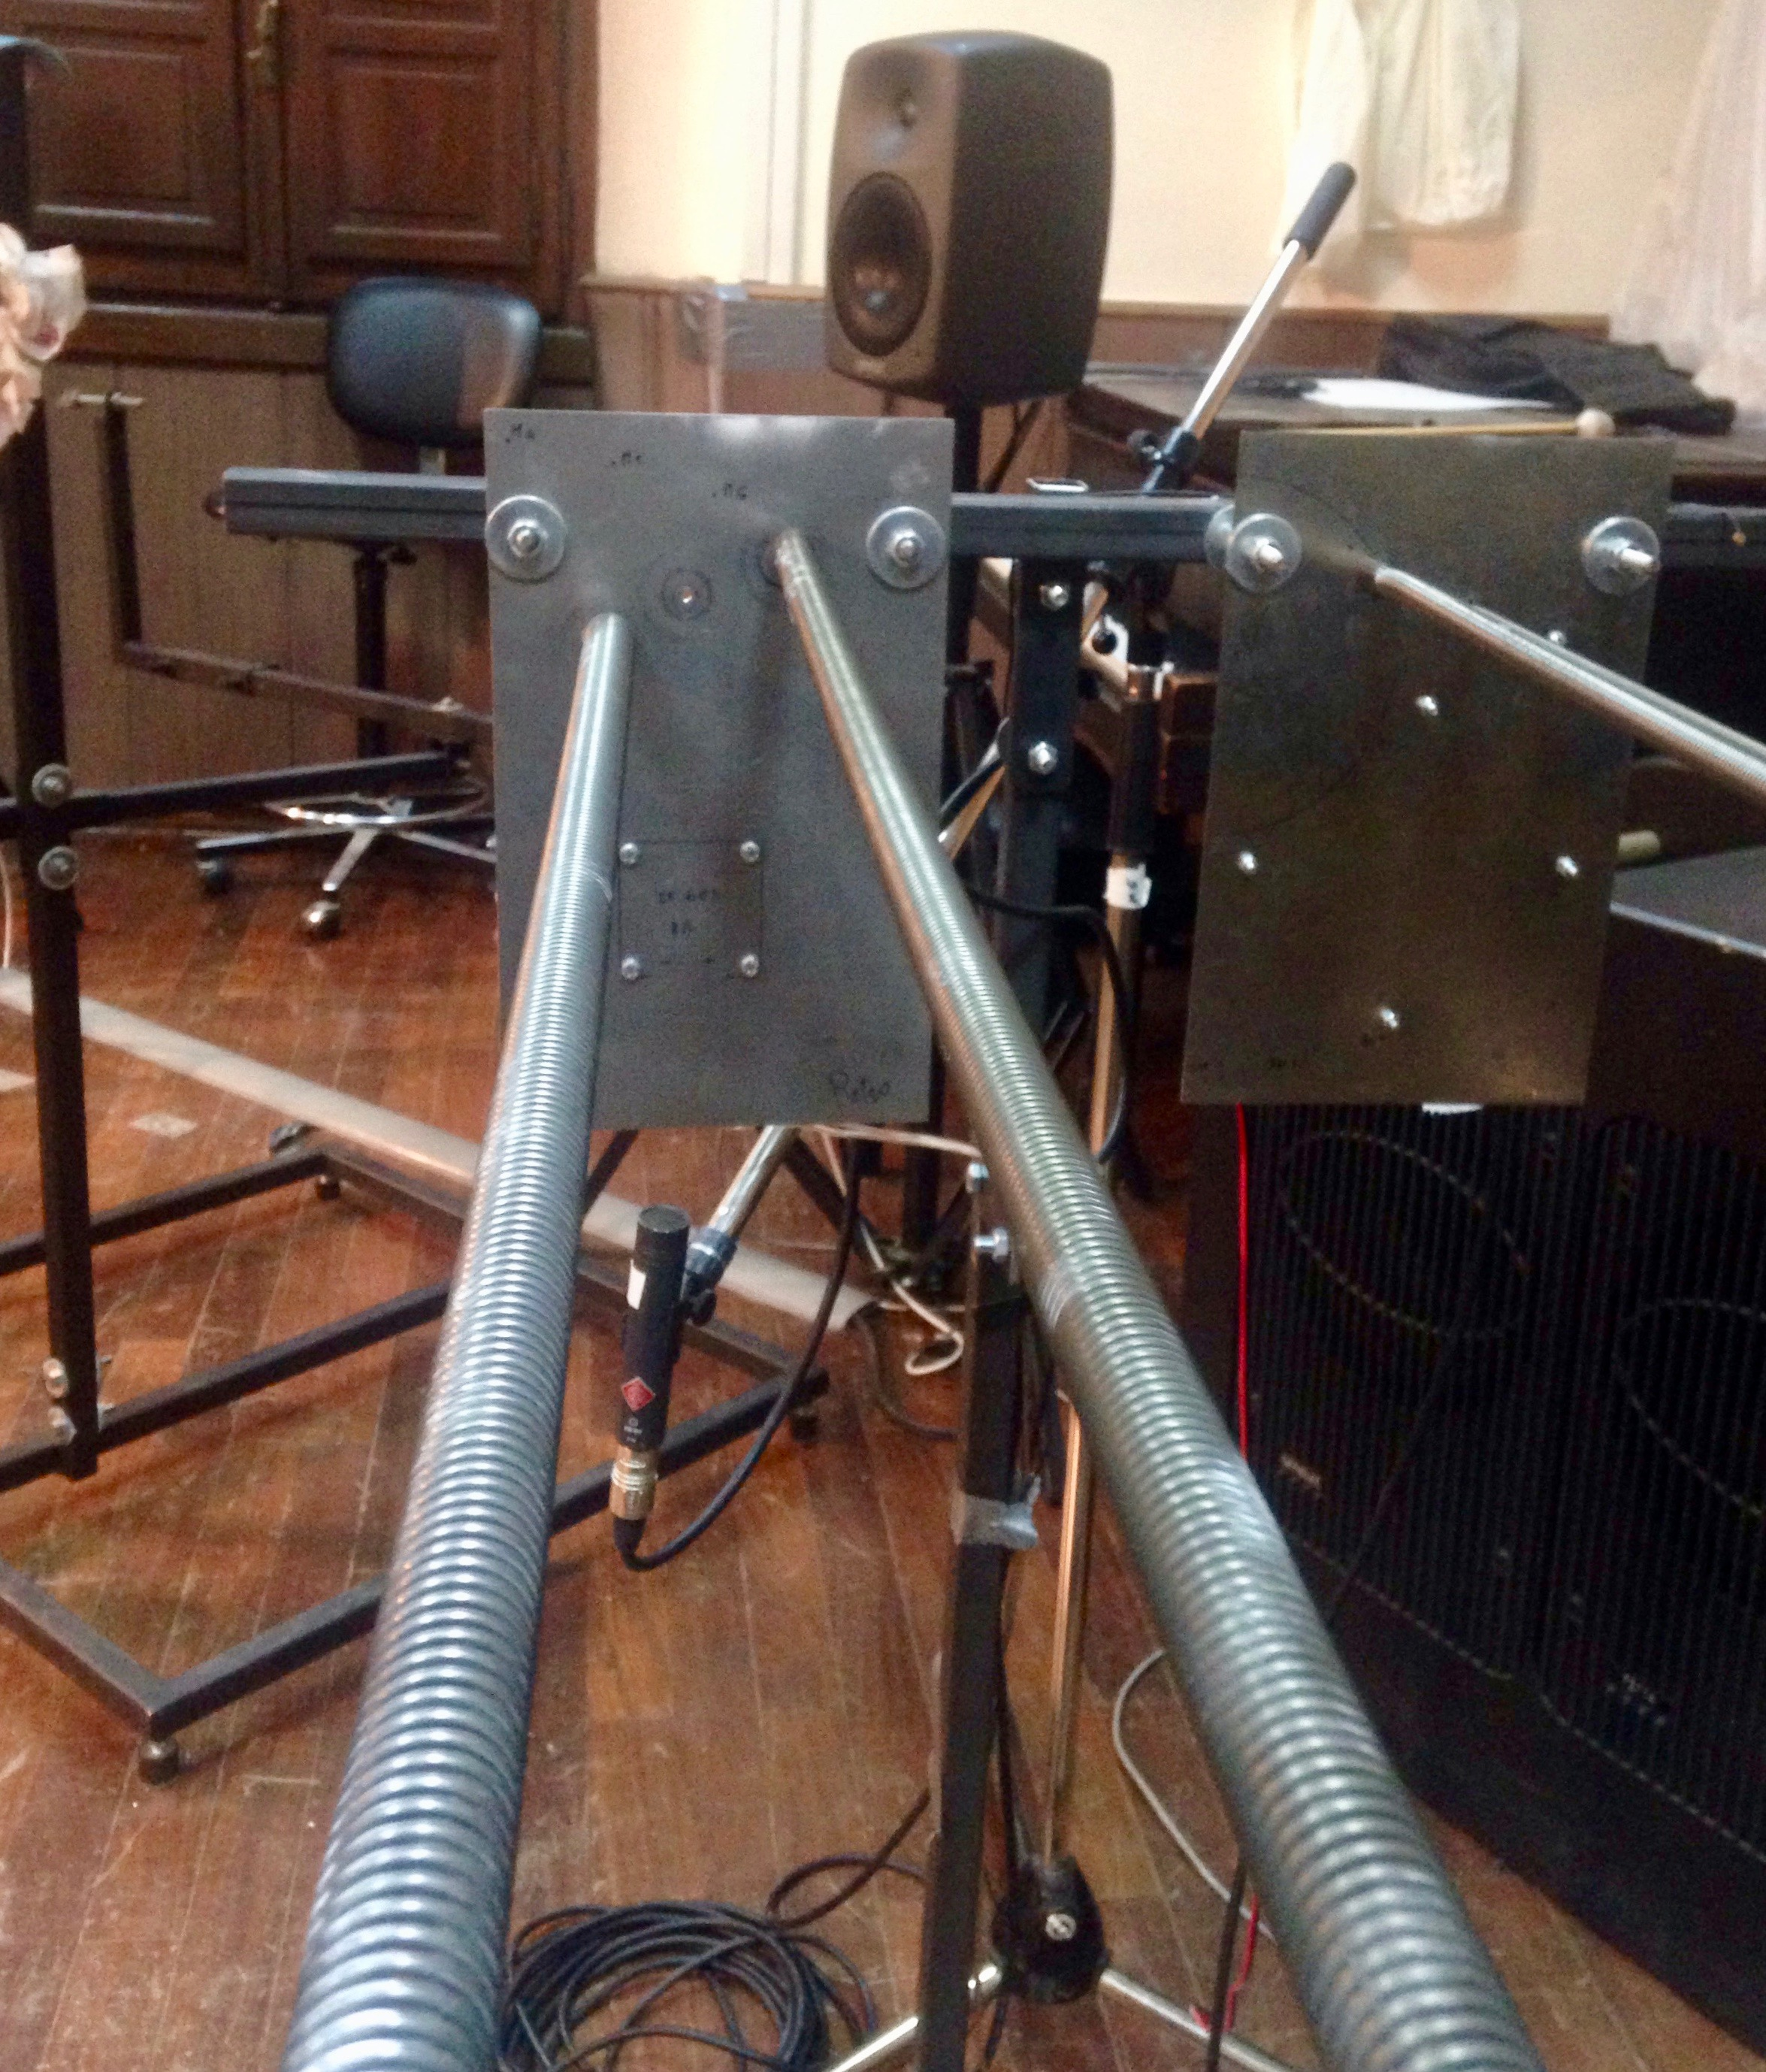
\includegraphics[width=.99\textwidth]{Spire2cc.jpg}
\caption{\textit{Sp.I.R.E.}, particolare della sezione più grave (Molla 5-4)}
\label{default}
\end{center}
\end{figure}
Le molle sono disposte sulle placche in due sezioni a gradini (\textit{fig. 13}) come se si andasse a suonare un violoncello, o un contrabbasso in posizione orizzontale. Durante la creazione di questo primo prototipo ho voluto utilizzare solo cinque molle per un'esigenza timbrica: alcune molle di diametro maggiore a scontrarsi, altre di diametro simile avevano la stessa risultante timbrica. 
\begin{figure}[htbp]
\begin{center}
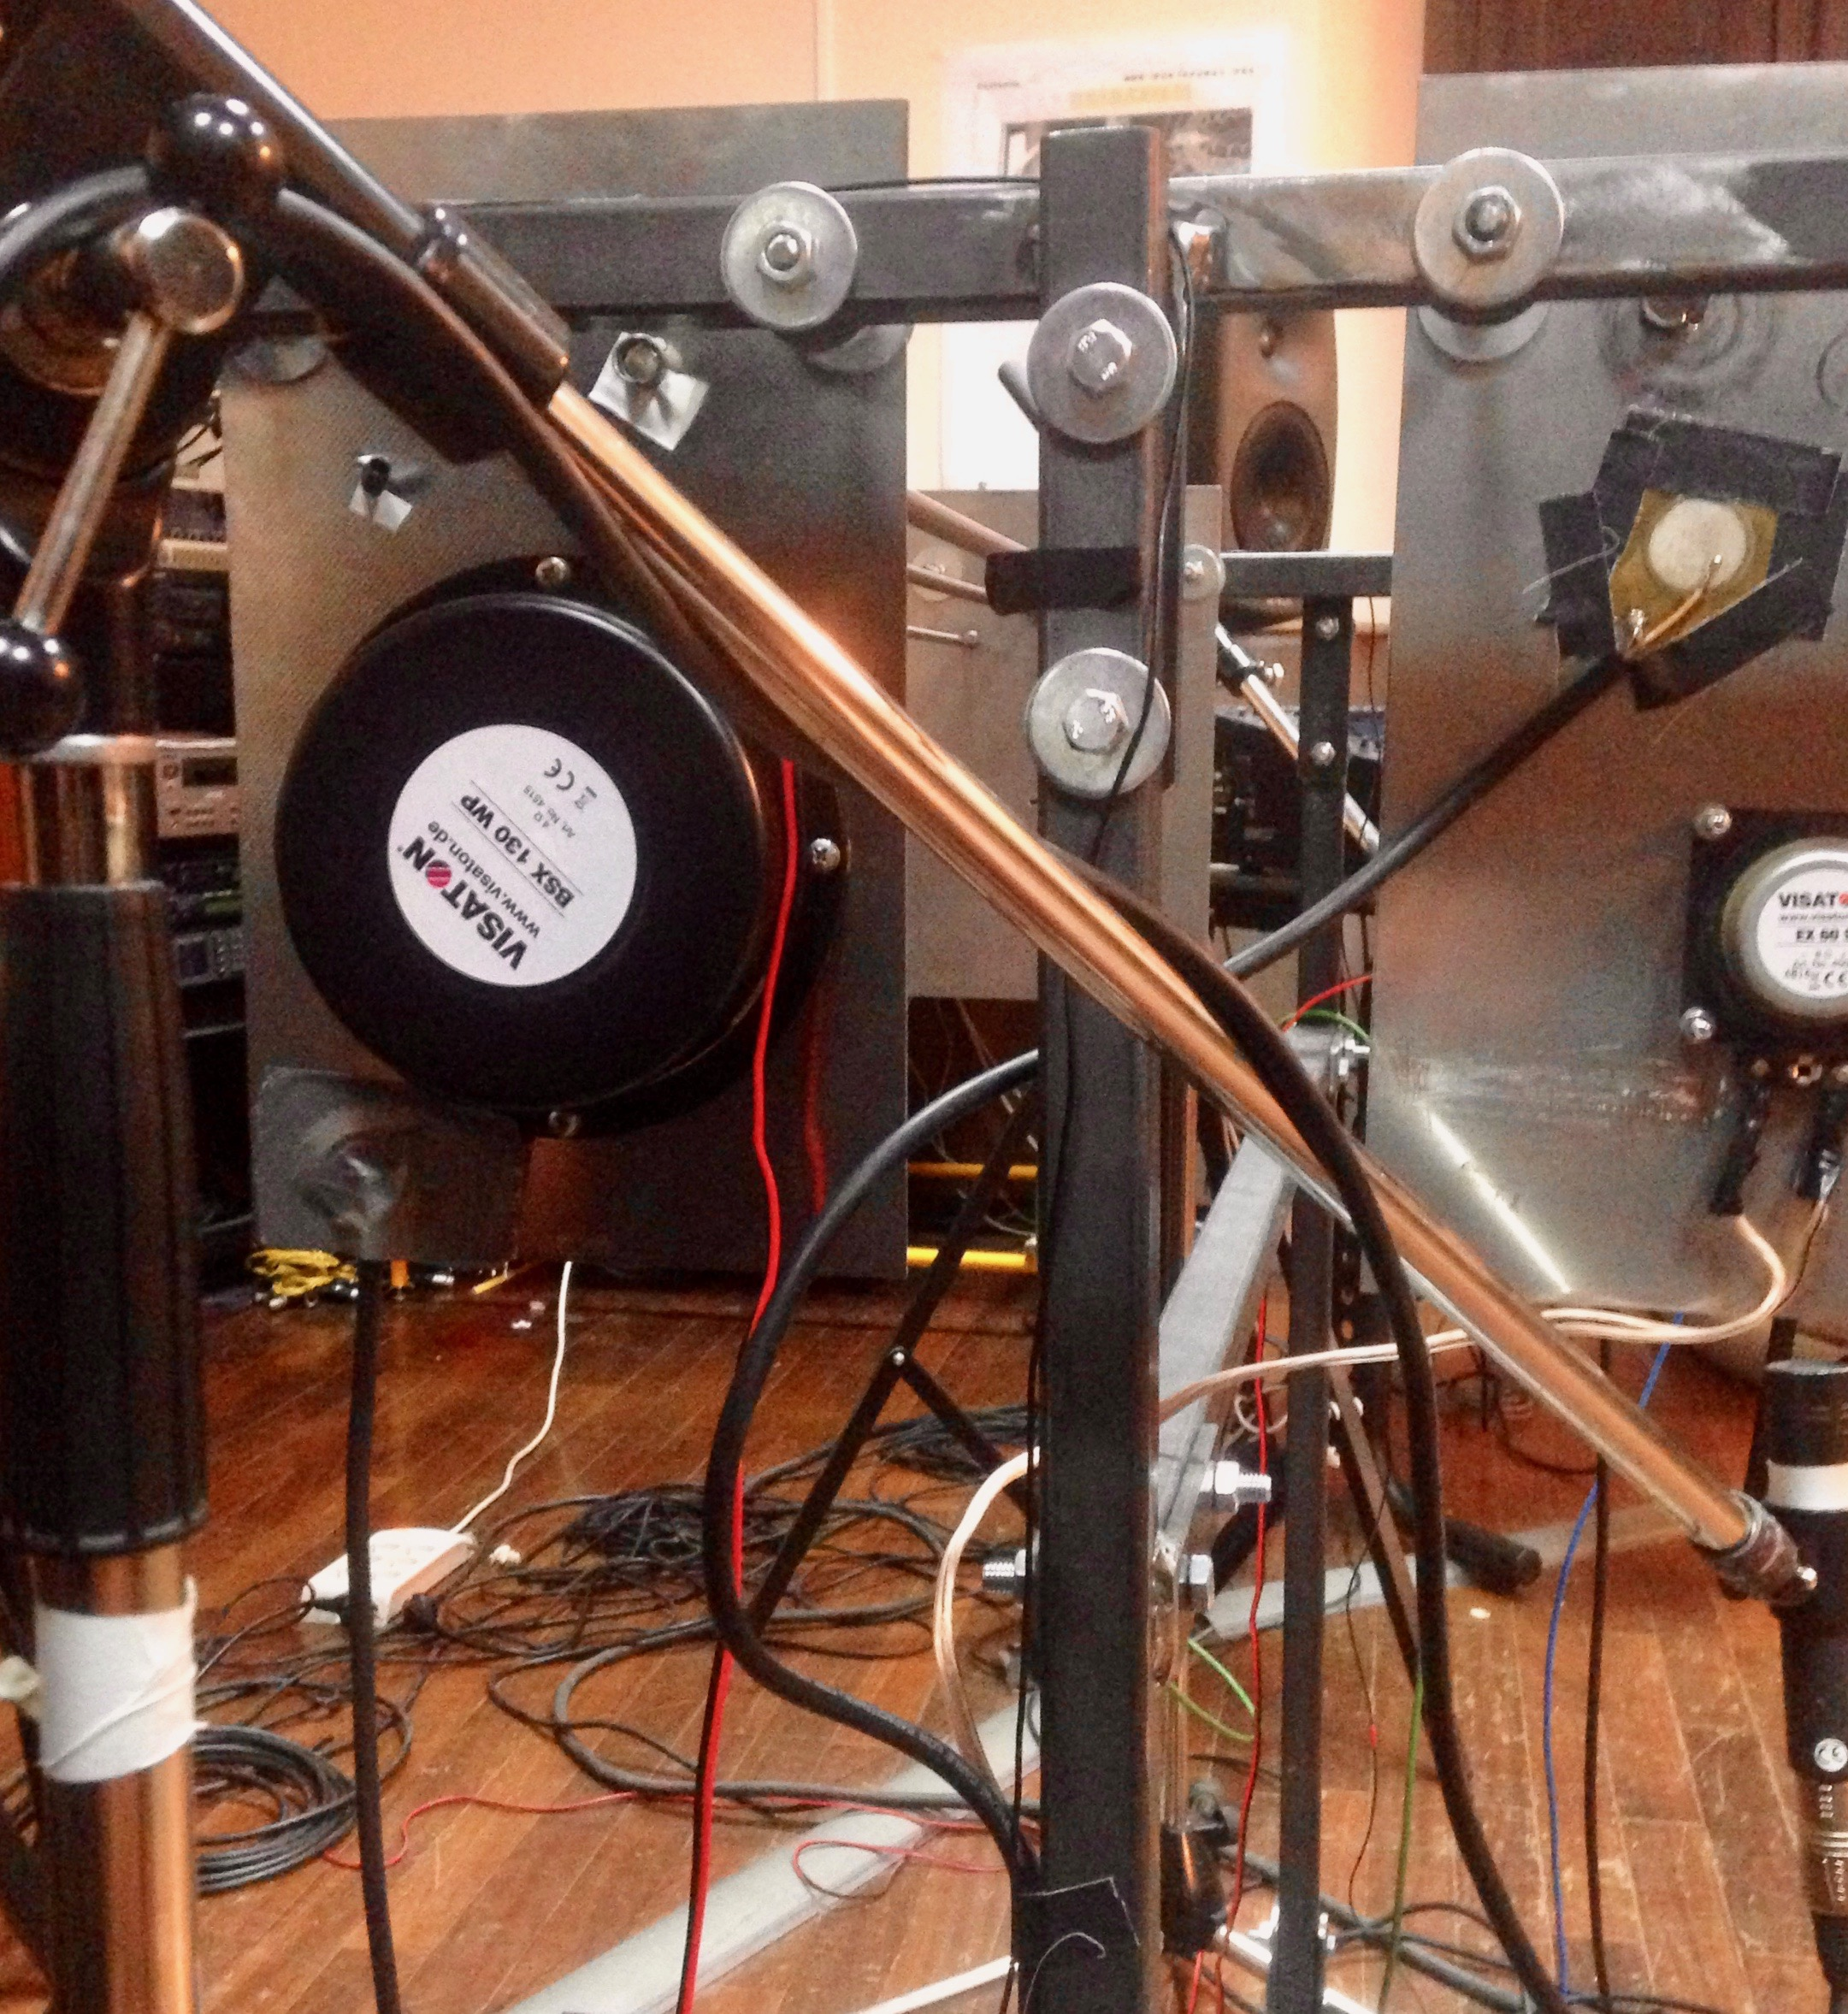
\includegraphics[width=.99\textwidth]{Spire1cc.jpg}
\caption{particolare attuatori BSX e ESX60}
\label{default}
\end{center}
\end{figure}
Gli attuatori sono stati fissati preventivamente tramite del nastro su una delle piastre di metallo e fatte delle prove di risposta del materiale risuonante. Trovato eccellente la risposta del metallo, in questo caso ferro e ferro zigrinato, sono stati segnati dei punti di ancoraggio degli attuatori, tramite viti con rondelle e bulloni.



\begin{tabular}{cp{2cm}p{2cm}p{2cm}} \textbf{Tipologia}&\textbf{ATTACCO}&\textbf{BATTENTE}&\textbf{Risposta}\\
\hline \textbf{METALLI}\\
\hline Placche metallo&8&Risonatori&Ottima\\
\hline Molle a trazione Inox&2&Strumento&Sufficiente\\
\hline Molle a trazione Acciaio armonico&6&Strumento&Ottima\\
\hline Tubo Quadrato Ferro&2&Basamento&Ottima\\
\hline Viti per innesti&Varie&Bas. Attuatori&Ottima\\
\hline \textbf{MOLLE}\\
\hline BSX 130 WP - 4 Ohm&4&Vibrazione Placca&Ottima\\
\hline ESX 45 - 8 Ohm&4&Vibrazione Placca&Sufficiente\\
\hline ESX 60 - 8 Ohm&3&Vibrazione Placca&Buona\\
\hline \textbf{MAGNETI}\\
\hline Humbucker&2&Amplificazione Molle&Buona\\
\hline Double Coil Bass&1&Amplificazione Molle&Ottima\\
\hline \textbf{PIEZOELETTRICI} \\
\hline Piezoelettrici&4&Amplificazione Molle&Buona\\
\hline
\end{tabular}

\section{Schema Elettrico}
Di seguito, lo schema elettrico per il collegamento degli attuatori:

\begin{figure}
\begin{center}
\includegraphics[width=.99\textwidth]{Elettrico.jpg}
\caption{Lo schema elettrico per il collegamento degli attuatori}
\label{default}
\end{center}
\end{figure}
